\chapter{Introduction}

\section{Kubernetes}

In this section we will dive into the topic of Kubernetes. We start by shortly overviewing the Kubernetes architecure. Then we expand on the Kubernetes resources, their kinds and their role in the target application environment. Finally, we consider the security of Kubernetes.

\subsection{Overview}

Kubernetes, also known as K8s, is an open source system for automating deployment, scaling, and management of containerized applications. It groups containers that make up an application into logical units for easy management and discovery. Kubernetes builds upon 15 years of experience of running production workloads at Google, combined with best-of-breed ideas and practices from the community. \cite{kubernetes}.

IBM defines Kubernetes as an open source \textbf{container orchestration platform} for scheduling and automating the deployment, management and scaling of containerized applications. Today, Kubernetes and the broader ecosystem of container-related technologies have merged to form the building blocks of modern cloud infrastructure. This ecosystem enables organizations to deliver a highly productive hybrid multicloud computing environment to perform complex tasks surrounding infrastructure and operations. It also supports cloud-native development by enabling a build-once-and-deploy-anywhere approach to building applications. \cite{ibm-kubernetes}.

It is important to emphasize that the Kubernetes abstracts the actual machines (nodes) from the user. Nodes can be physical on-premises servers, or VMs that reside either on-premises or at a cloud provider. Kubernetes takes on the responsibilty of figuring out the deployment target for a particular application. That is, user only defines the desired state of the infrastructure using YAML or JSON configuration files. Kubernetes then creates all the workloads based on the applied configuration.

\subsection{Kubernetes Architecture}

While Kubernetes requires at least three nodes to run, there are some implementation designed for the local use, which emulate this concept (see Subsection~\ref{sec:other-kubernetes-implementations}). The master node is called control plane. The control plane manages the worker nodes and the Pods in the cluster. In production environments, the control plane usually runs across multiple computers and a cluster usually runs multiple nodes, providing fault-tolerance and high availability. Worker nodes host the actual workload inside the cluster. Figure~\ref{img:kubernetes-architecture} provides a simple high-level overview of a typical Kubernetes cluster with a Control Plane and three worker nodes.

\begin{figure}[!hbt]
	\begin{center}
		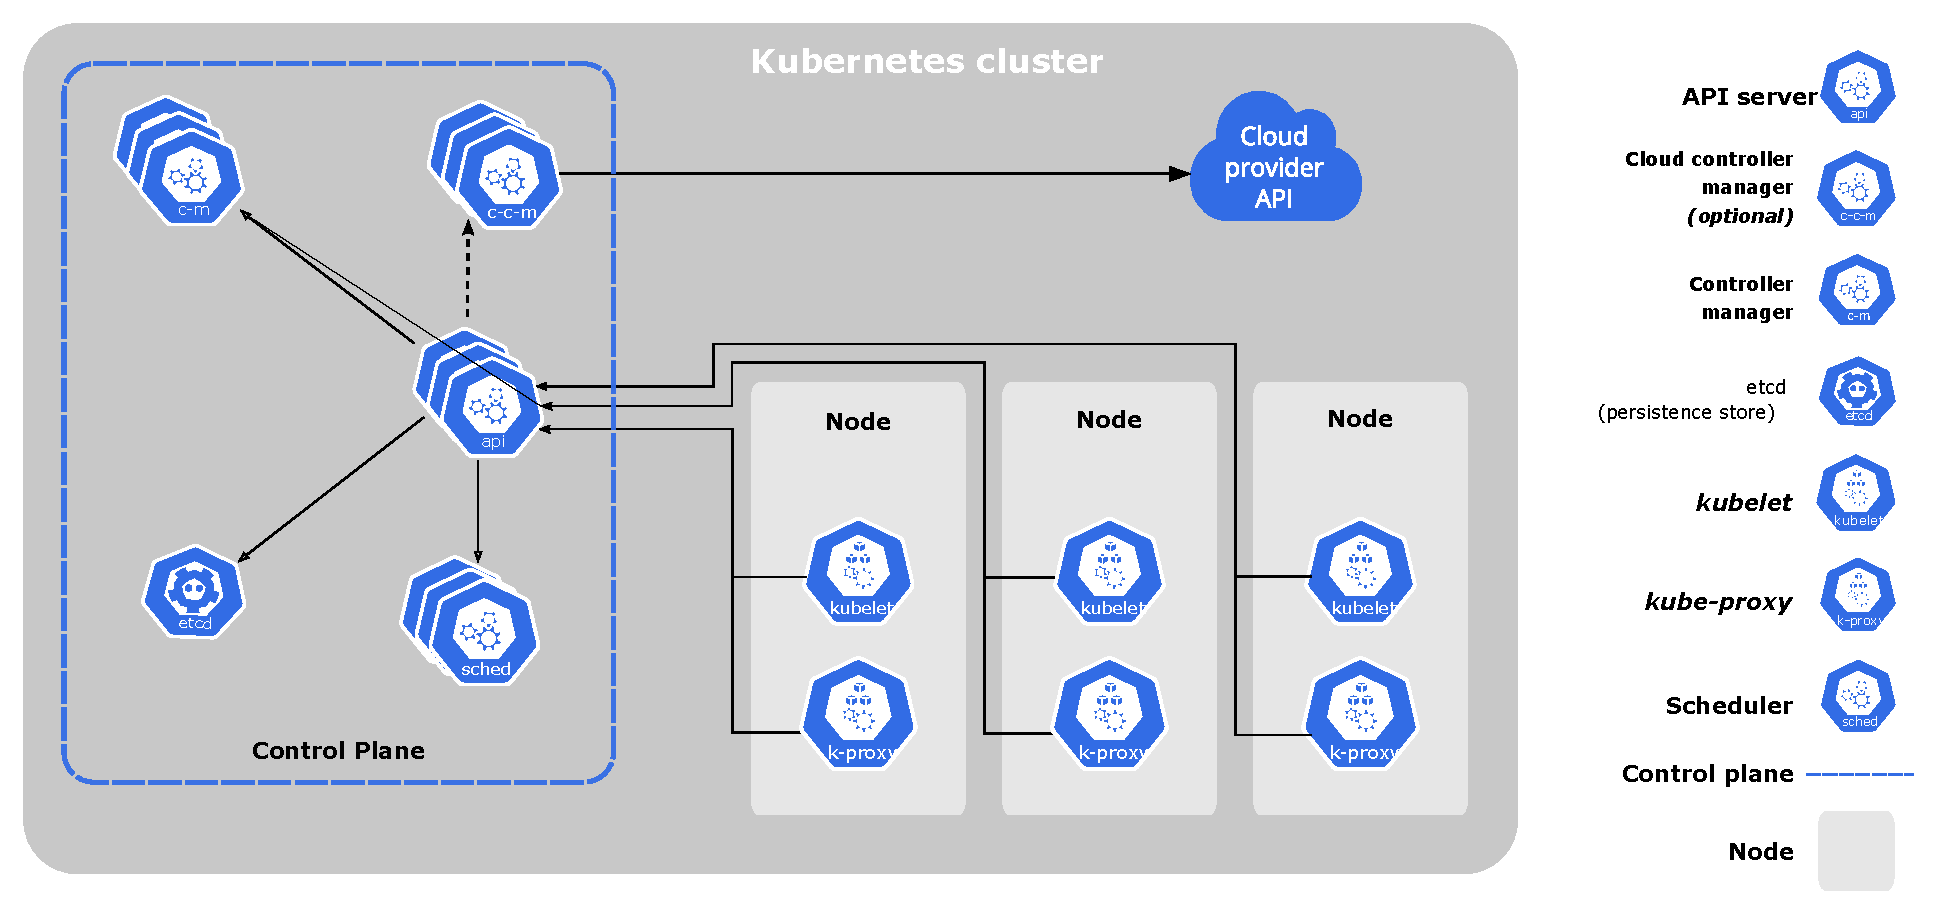
\includegraphics[width=0.85\textwidth]{images/components-of-kubernetes.pdf}
        \caption{Kubernetes cluster architecure overview with its main components.}
		\label{img:kubernetes-architecture}
	\end{center}
\end{figure}

\subsubsection*{Control Plane overview}

Control plane runs the following components: 
\begin{itemize}
\item \textbf{kube-apiserver} \\
Kube-apiserver exposes the Kubernetes API, which is acting as a frontend for the Kubernetes control plane.
\item \textbf{etcd} \\
Etcd is a key-value store, where all of the cluster data is stored.
\item \textbf{kube-scheduler} \\
Each time a new pod is created, it is passed to the kube-scheduler, which assigns the pod to the specific node to run on (based on individual and collective resource requirements, hardware/software/policy constraints, affinity and anti-affinity specifications, data locality, inter-workload interference, and deadlines).
\item \textbf{kube-controller-manager} \\
Each Kubernetes resource has its own controller (e.g. NodeController, JobController, ServiceAccountController); all of them are compiled as one binary called kube-controller-manager.
\item \textbf{cloud-controller-manager} \\
Cloud-controller-manager embeds cloud-specific control logic. It differs depending on the cloud provider or can be absent completely, when running Kubernetes locally.
\end{itemize}

\subsubsection*{Worker Node overview}

Each worker node has a kubelet and kube-proxy installed. Kubelet is an agent that manages runnning pods and containers. Kube-proxy is a network proxy that implements parts of the Kubernetes service concept. It maintains network rules on nodes, making in- outside-cluster communitcation possible.

Then, of course, each worker node has a set of running pods. A typical use would involve multiple running applications. Depending on the size of the node and the application resoucre consumption it can accomodate on average from one to a few dozens applications with various business purposes.

\subsection{Kubernetes Resources}

Kubernetes resources are fundamental components that define various entities within a Kubernetes cluster. Resources are objects that represent the desired state and configuration of the infrastructure, applications, and services running on the cluster. Kubernetes provides a range of resources that enable developers and operators to define, manage, and scale containerized applications, network policies, storage requirements, and more. These resources are defined declaratively in YAML or JSON files, which makes infrastructure setup consistent and reproducible.

Among key Kubernetes resoucres are:
\begin{itemize}
    \item \textbf{Pods} \\
        Pod is the atomic workload unit in the Kubernetes cluster. It encapsulates one or more containers that share the same network. It represents a single instance of a running application.
    \item \textbf{Deployments} \\
        Deployments are a higher level of abstraction for the Pods. They allow to define replica count and rollout/rollback strategy for the updates, which can be used to ensure availability for the application.
    \item \textbf{Services} \\
        Services provide a communication layer for the pods inside one cluster. Being an abstraction over the pods' network, they provide reliable access to the selected workloads, while serving as a Load Balancer. 
    \item \textbf{ConfigMaps} and \textbf{Secrets} \\
        ConfigMaps and Secrets allow users to store data outside the workload. ConfigMaps are usually used to store non-sensitive information like environment and application configuration parameters. Secrets are a more secure resource designed for API keys, passwords and other sensitive data.
    \item \textbf{PersistentVolumes} and \textbf{PersistentVolumeClaims} \\
        These resources enable stateful applications to request and mount durable storage within a cluster, allowing data to persist independently of the Pod lifecycle.
\end{itemize}

Above are the most commonly used resources, which we also leverage in the practical part of the paper. Therefore, it is important that the reader understands the position and the purpose of each resource in the cluster infrastructure.

\subsubsection*{Workloads}

Minimal computing units in Kubernetes are Containers, which are running in Pods. However, to simplify the management of Pods, Kubernetes has workload resources, which manage the set of Pods. They make sure the desired number of Pods of right kind are running to match the declaration.

Deployments and ReplicaSets are a good fit for stateless applications. Each pod in the Deployment is interchangebeable. Deployments are easily scalable and have built-in versioning and rollout mechanisms.

StatefulSet allows to create sets of stateful applications. They might share the same PersistentVolume and replicate data between each other.

DaemonSet defines Pods that provide node-local facilities. These might be fundamental to the operation of your cluster, such as a networking helper tool, or be part of an add-on.

Job and CronJob define tasks that run to completion and then stop. Jobs represent one-off tasks, whereas CronJobs recur according to a schedule.

\subsubsection*{Networking}

Kubernetes networking model makes Pods look like VMs in the networking aspect. Pods on any nodes can communicate with each other without NAT. Containers inside the same Pod share its network meaning that they can reach each other using localhost.

Kubernetes networking addresses four concerns:
\begin{itemize}
\item Containers within a Pod use networking to communicate via loopback.
\item Cluster networking provides communication between different Pods.
\item The Service API lets you expose an application running in Pods to be reachable from outside your cluster.
\item Ingress provides extra functionality specifically for exposing HTTP applications, websites and APIs.
\item You can also use Services to publish services only for consumption inside your cluster.
\end{itemize}

\subsubsection*{Storage}

Kubernetes does not ship a particular implementation of storage. However, it provides a range of resources that define the storage concept and supports different types of volumes. A Pod can use any number of volume types simultaneously. Ephemeral volume types have a lifetime of a pod, but persistent volumes exist beyond the lifetime of a pod. When a pod ceases to exist, Kubernetes destroys ephemeral volumes; however, Kubernetes does not destroy persistent volumes. For any kind of volume in a given pod, data is preserved across container restarts.

At its core, a volume is a directory, possibly with some data in it, which is accessible to the containers in a pod. How that directory comes to be, the medium that backs it, and the contents of it are determined by the particular volume type used.

PersistentVolumes and PersistentVolumeClaims are the resources kinds most important to understand here.
\begin{itemize}
\item A PersistentVolume (PV) is a piece of storage in the cluster that has been provisioned by an administrator or dynamically provisioned using Storage Classes. It is a resource in the cluster just like a node is a cluster resource. PVs are volume plugins like Volumes, but have a lifecycle independent of any individual Pod that uses the PV. This API object captures the details of the implementation of the storage, be that NFS, iSCSI, or a cloud-provider-specific storage system.
\item A PersistentVolumeClaim (PVC) is a request for storage by a user. It is similar to a Pod. Pods consume node resources and PVCs consume PV resources. Pods can request specific levels of resources (CPU and Memory). Claims can request specific size and access modes (e.g., they can be mounted ReadWriteOnce, ReadOnlyMany or ReadWriteMany). Once and Many here refer to a number of Pods that can perform the read or write simultaneously.
\end{itemize}

\subsection{Infrastructure Security}

When we are talking about the infrastructure security, we must consider multiple layers. Going from the top to the bottom, we start with the security measurements taken on the Cloud provider side. In most cases this is not something we can affect and the security of different Cloud providers varies significantly. Unfortunately, this is out of scope of this paper, but all of the "big five" Cloud providers (AWS, Azure, Google Cloud, Alibaba and IBM) maintain high security standarts and security risks generally should not be a concern for their end users. Then, we get to the cluster itself. On the cluster level we must consider the security of the nodes, security of the cluster components and their configuration. At this layer we have already some space for the misconfigurations to appear. Here we can evaluate the security of the single components using some of the security scanners presented in \nameref{sec:kubernetes-security-automation}. Lastly, we get to the application level, where the security of the application code, Kubernetes resoucre configuration, libraries, dependencies and base images is the main concern. Again, this is the layer, where the developers have the most access to, thus, providing a lot of space for the possibility of a human error. In this paper we mostly work on this level when we do our research.

Officially, The Linux Foundation provides only some security guidelines for each of the layers. However, bundled with Kubernetes we get a few means to keep the security under control. Below we present an overview of the Kubernetes security recommendations, RBAC and Data security inside Kubernetes.

\subsubsection*{Kubernetes security recommendations}

This section gathers the official security recommendations provided by the Kubernetes. They provide a list of concerns for each level of the cloud infrastructure. Cloud infrastructure can be viewed as a composition of four layers as displayed by the Figure~\ref{img:cloud-security}.

\begin{figure}[!hbt]
	\begin{center}
		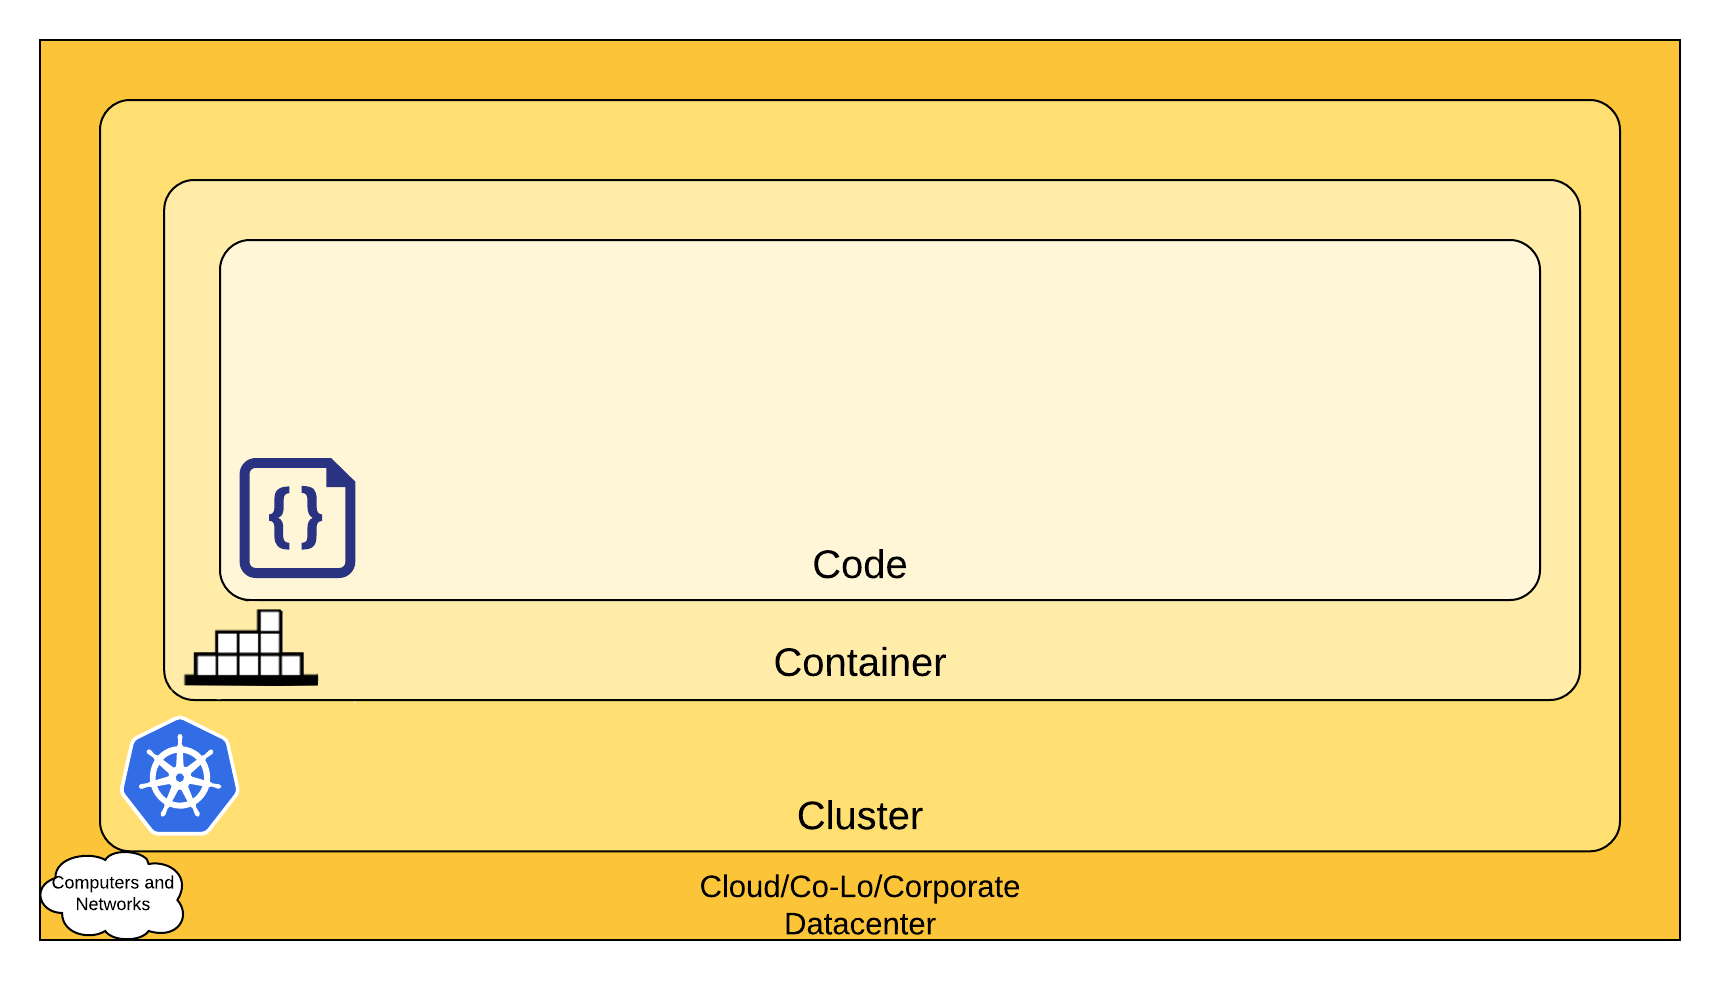
\includegraphics[width=0.75\textwidth]{images/cloud-security.png}
        \caption{Four layers of the cloud infrastructure.}
		\label{img:cloud-security}
	\end{center}
\end{figure}

Each layer is built upon the previous one and its security depends on the security of the outer layers. It is, therefore, important to maintain high security standarts on base levels (Cloud, Cluster, Container).

\begin{enumerate}

\item \textbf{Cloud} \\
Each cloud provider has its own security policies and guidelines. There are, however, some general infrastructure-level security best advice described by in the Table~\ref{tab:cloud-security-recommendations}.

\begin{table}[H]
    \begin{center}
        \begin{tabular}{ | p{.20\textwidth} | p{.80\textwidth} | } 
         \hline
         \textbf{Area of Concern for Kubernetes Infrastructure} & \textbf{Recommendation} \\ 
         \hline
         Network access to API Server (Control plane) & All access to the Kubernetes control plane is not allowed publicly on the internet and is controlled by network access control lists restricted to the set of IP addresses needed to administer the cluster. \\ 
         \hline
         Network access to Nodes (nodes)  & Nodes should be configured to only accept connections (via network access control lists) from the control plane on the specified ports, and accept connections for services in Kubernetes of type NodePort and LoadBalancer. If possible, these nodes should not be exposed on the public internet entirely. \\ 
         \hline
         Kubernetes access to Cloud Provider API & Each cloud provider needs to grant a different set of permissions to the Kubernetes control plane and nodes. It is best to provide the cluster with cloud provider access that follows the principle of least privilege for the resources it needs to administer. \\
         \hline
         Access to etcd & Access to etcd (the datastore of Kubernetes) should be limited to the control plane only. Depending on your configuration, you should attempt to use etcd over TLS. \\
         \hline
         etcd Encryption & Wherever possible it's a good practice to encrypt all storage at rest, and since etcd holds the state of the entire cluster (including Secrets) its disk should especially be encrypted at rest. \\
         \hline
        \end{tabular}
    \end{center}
    \caption{Security recommendations for the Cloud layer.}
    \label{tab:cloud-security-recommendations}
\end{table}

\item \textbf{Cluster} \\
There are two cluster security concerns that could be addressed: securing the configurable cluster components and securing the applications running in the cluster.

There are a few things to consider regarding the application security:
\begin{itemize}
\item RBAC Authorization (Access to the Kubernetes API)
\item Authentication	
\item Application secrets management (and encrypting them in etcd at rest)
\item Ensuring that pods meet defined Pod Security Standards
\item Quality of Service (and Cluster resource management)
\item Network Policies
\item TLS for Kubernetes Ingress
\end{itemize}

\item \textbf{Container} \\
Securing containers is a vast topic, which deserves its own chapter. There are, nevertheless, a few general recommendation provided by the Kubernetes, which you can find in the Table~\ref{tab:container-security-recommendations}.

\begin{table}[H]
    \begin{center}
        \begin{tabular}{ | p{.20\textwidth} | p{.80\textwidth} | } 
        \hline
        \textbf{Area of Concern for Containers} & \textbf{Recommendation} \\ 
        \hline
        Container Vulnerability Scanning and OS Dependency Security & As part of an image build step, you should scan your containers for known vulnerabilities. \\ 
        \hline
        Image Signing and Enforcement & Sign container images to maintain a system of trust for the content of your containers. \\ 
        \hline
        Disallow privileged users & When constructing containers, create users inside of the containers that have the least level of operating system privilege necessary in order to carry out the goal of the container. \\
        \hline
        \end{tabular}
    \end{center}
    \caption{Security recommendations for the Container layer.}
    \label{tab:container-security-recommendations}
\end{table}

\item \textbf{Code} \\
When it comes to code, the developers have the most flexibility to design secure applications. There are a lot of issues to address, which may vary significantly from application to application depending on its purpose, architecture and framework base. Kubernetes documentation gives a handful of recommendations regarding this topic, which are displayed below in the Table~\ref{tab:code-security-recommendations}.

\begin{table}[H]
    \begin{center}
        \begin{tabular}{ | p{.20\textwidth} | p{.80\textwidth} | } 
        \hline
        \textbf{Area of Concern for Code} & \textbf{Recommendation} \\ 
        \hline
        Access over TLS only & If your code needs to communicate by TCP, perform a TLS handshake with the client ahead of time. With the exception of a few cases, encrypt everything in transit. Going one step further, it's a good idea to encrypt network traffic between services. This can be done through a process known as mutual TLS authentication or mTLS which performs a two sided verification of communication between two certificate holding services. \\ 
        \hline
        Limiting port ranges of communication & This recommendation may be a bit self-explanatory, but wherever possible you should only expose the ports on your service that are absolutely essential for communication or metric gathering. \\ 
        \hline
        3rd Party Dependency Security & It is a good practice to regularly scan your application's third party libraries for known security vulnerabilities. Each programming language has a tool for performing this check automatically. \\
        \hline
        Static Code Analysis & Most languages provide a way for a snippet of code to be analyzed for any potentially unsafe coding practices. Whenever possible you should perform checks using automated tooling that can scan codebases for common security errors. \\
        \hline
        Dynamic probing attacks & There are a few automated tools that you can run against your service to try some of the well known service attacks. These include SQL injection, CSRF, and XSS. One of the most popular dynamic analysis tools is the OWASP Zed Attack proxy tool. \\
        \hline
        \end{tabular}
    \end{center}
    \caption{Security recommendations for the Code layer.}
    \label{tab:code-security-recommendations}
\end{table}
                      
\end{enumerate}

\subsubsection*{Role Based Access Control}

\subsubsection*{Data security}

\subsection{Other Kubernetes Implementations}
\label{sec:other-kubernetes-implementations}

\subsubsection*{Openshift}

\subsubsection*{Rancher Desktop}
%\section{Deep learning}
% something about deep learning 
    % convolutional neural network
        % convolutional layers, pooling, FC
    % maybe about resnet if I wanna compare it
    

Solving mathematical problems is a very easy task for computers. However, the real challenge is to solve problems that are natural to humans but cannot be formally described by a set of rules for computers. Things like understanding spoken words, recognizing objects, or identification of people are all instinctively learned by humans and require years of experience. For computers to gain this knowledge, a similar concept is used. They also learn from experience by using a large amount of provided data. The system of learning is based on a hierarchy of concepts, where each concept is built upon relations with simpler concepts. Drawing a graph of this hierarchy would result in a deep structure of concepts, which is where the name deep learning comes from \cite{Goodfellow-et-al-2016}.

In this section, we will talk about a specific type of deep learning technique - convolutional neural networks. 

\subsection{Convolutional neural network}

A convolutional neural network (CNN) is a specific type of neural network that operates on grid-like data. It is most commonly used when working with images, which are represented as a 2D grid of pixel values \cite{Goodfellow-et-al-2016}.

The process is the same as with a neural network, but the inner structure is different. The CNN receives the input, which is fed through the series of hidden layers and the final score is computed in the output layer. Each layer is made up of a set of neurons, which have learnable weights and biases. However, the neurons in CNN are arranged in 3 dimensions: width, height, and depth as is depicted in the Figure \ref{img:cnn0}.

\begin{figure}[h]
    \centering
    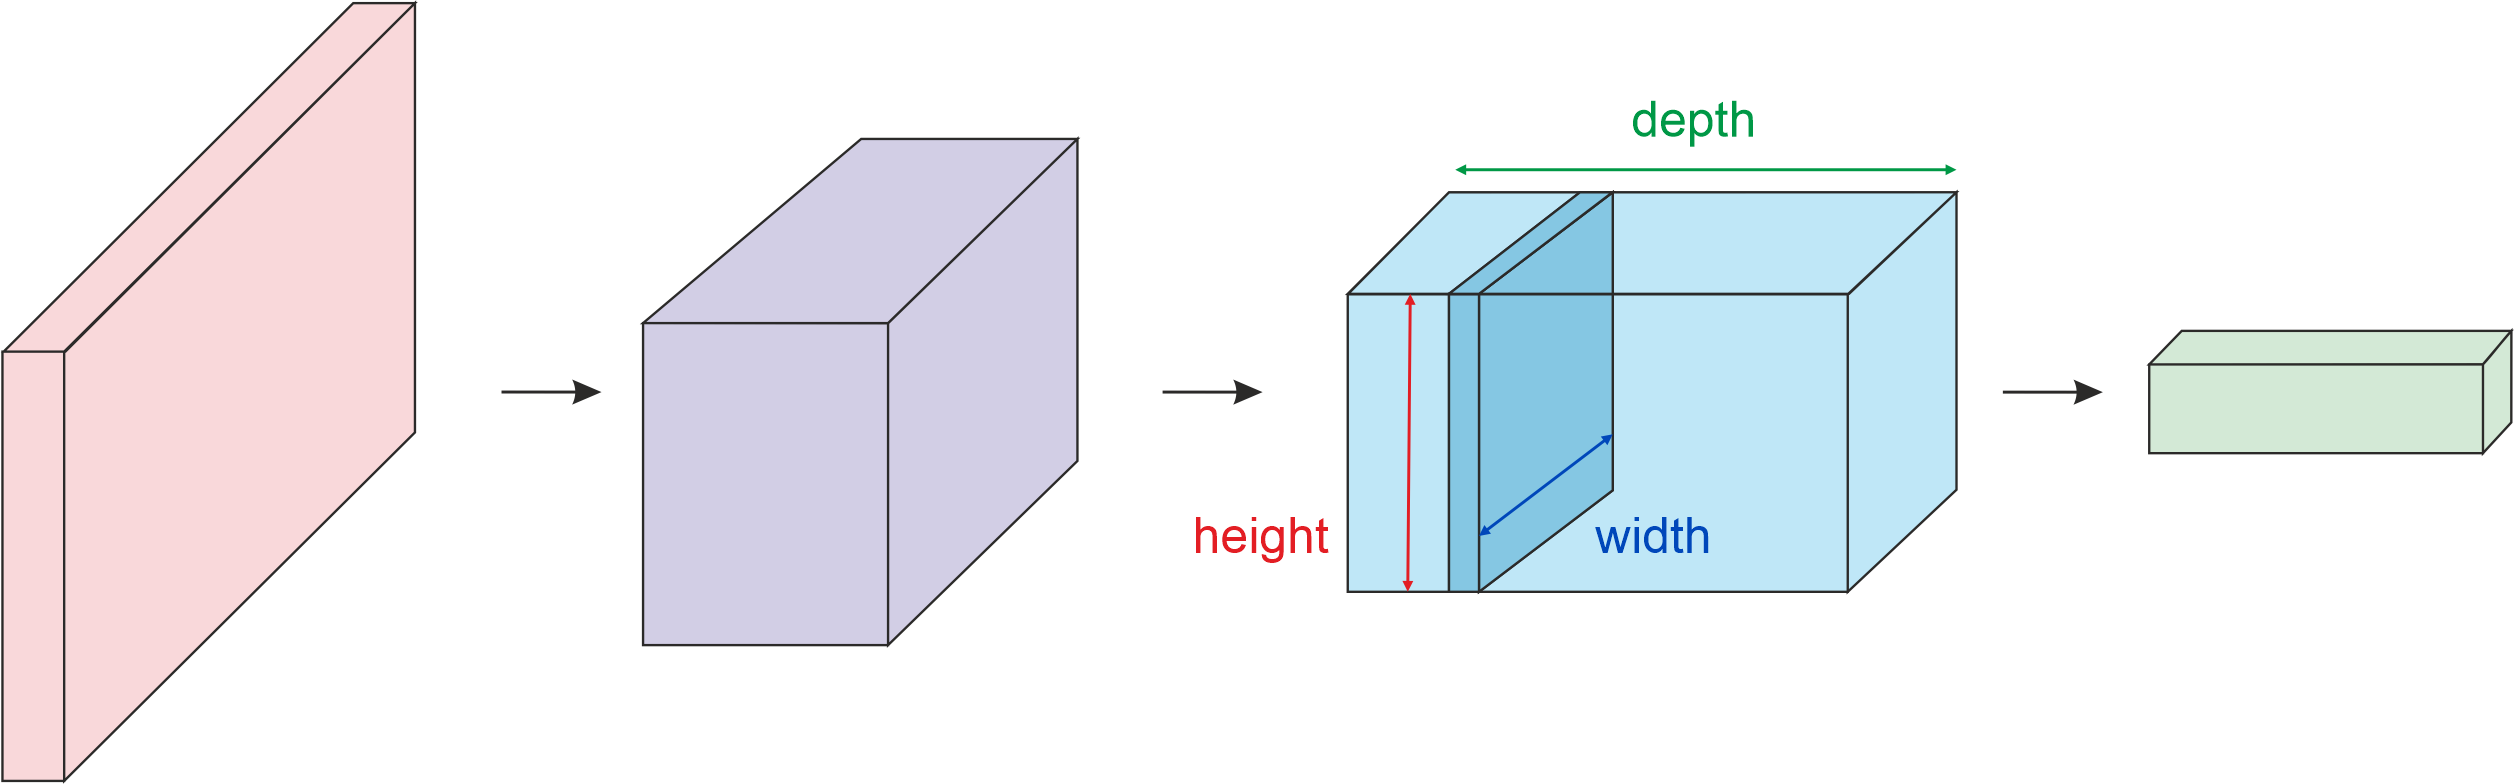
\includegraphics[width=.8\textwidth]{images/cnn.png}
    \caption{Inside structure of convolutional neural network.}
    \label{img:cnn0}
\end{figure}

%In neural networks, layers are fully connected, which means that each neuron from the previous layer is connected to each neuron in the following layer. 

While in neural networks, all layers are fully connected, the CNN has 3 main building blocks: convolutional layer, pooling layer, and fully connected layer \cite{standford}.

\subsubsection{Convolutional layer}

The convolutional layer is the most essential part of CNN and as the name suggests, this is where the convolution operation happens. Each convolutional layer has a defined set of filters/kernels. The filter has a significantly smaller spatial size than the input image (ranging from 3 to 10 pixels wide) but covers the full depth of the input. The values of each filter represent weights learned by the network \cite{standford}.

During the forward pass of the network, the convolution is applied to the input volume in a manner that each filter is moved across the width and height of the input. How many pixels the filter moves during convolution is defined by parameter stride. At each position, a dot product is computed between values of the filter and values of the input. This creates a 2D activation matrix also called a feature map. 
This way, each filter in the layer creates a feature map containing the response of that specific filter at each spatial position of the input. Stacking all these feature maps together builds the output volume of the layer, where the depth is the number of filters in the layer \cite{Goodfellow-et-al-2016} \cite{standford}.

Formally, the convolution is defined by the following formula:
\begin{equation}
    (K * I) (i,j) = \displaystyle\sum_{m}  \displaystyle\sum_{n} I(i - m, j - n) K(m, n).
\end{equation}
where K is the kernel, and I is the input volume \cite{Goodfellow-et-al-2016}.

A simple example of convolution applied to 2D input is shown in the Figure \ref{img:conv0}. It shows how the kernel is moved through the matrix with a stride 1 and how the dot product at each position is calculated. 

\begin{figure}[h]
    \centering
    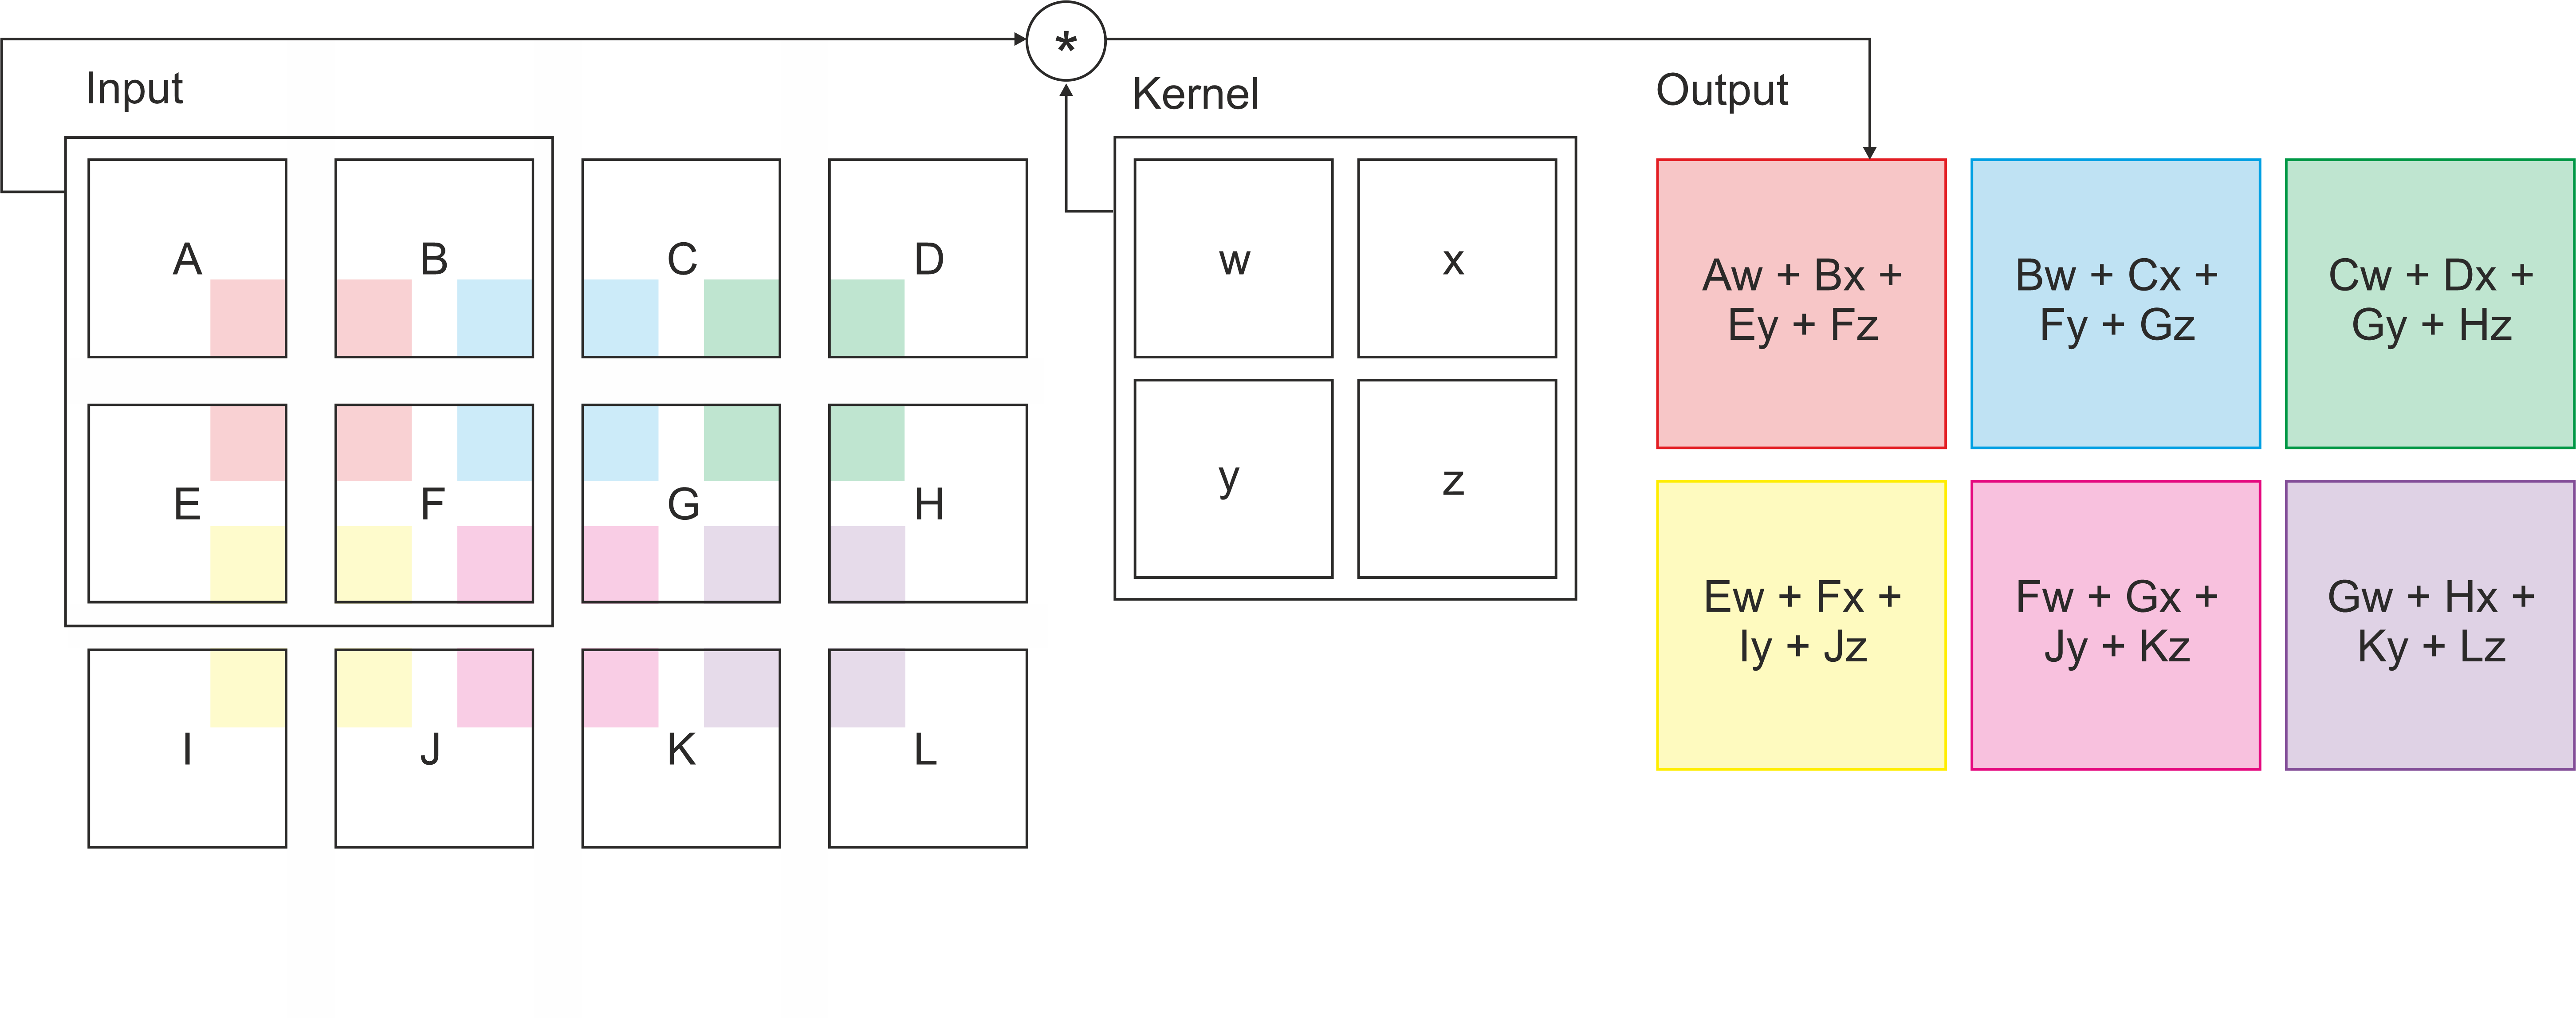
\includegraphics[width=.8\textwidth]{images/convolution3.png}
    \caption{An example of simple convolution.}
    \label{img:conv0}
\end{figure}

\subsubsection{Pooling layer}

Another important layer in the architecture of CNN is the pooling layer. It is useful for reducing the spatial size of feature maps and therefore makes the computation more effective as the network gets deeper. It is also helpful in keeping the representation approximately the same when the input image is slightly translated \cite{Goodfellow-et-al-2016}.

The pooling layer has a defined size of the kernel, which usually ranges from 2x2 to 3x3 pixels spatially. Another important parameter is the pooling function that is performed on the input. The most common is max pooling, but there are other popular pooling functions such as average, weighted average, or L2 norm pooling. 
Unlike other layers in the CNN, the pooling layer has no learnable parameters \cite{standford}.

Pooling is performed in a similar fashion as convolution. A kernel is moved across the input volume spatially but operates on each depth slice separately. This way only the spatial size of the input is reduced and the depth stays the same. At each spatial location, the output value is computed using the pooling function performed on the values of the input \cite{standford}.

The process of max pooling is illustrated in the Figure \ref{img:maxpool0}. The size of the kernel in the example is 2x2 with a stride of 2. It is common practice to use the stride the same size as the kernel if we do not want an overlapping pooling.  

\begin{figure}[h]
    \centering
    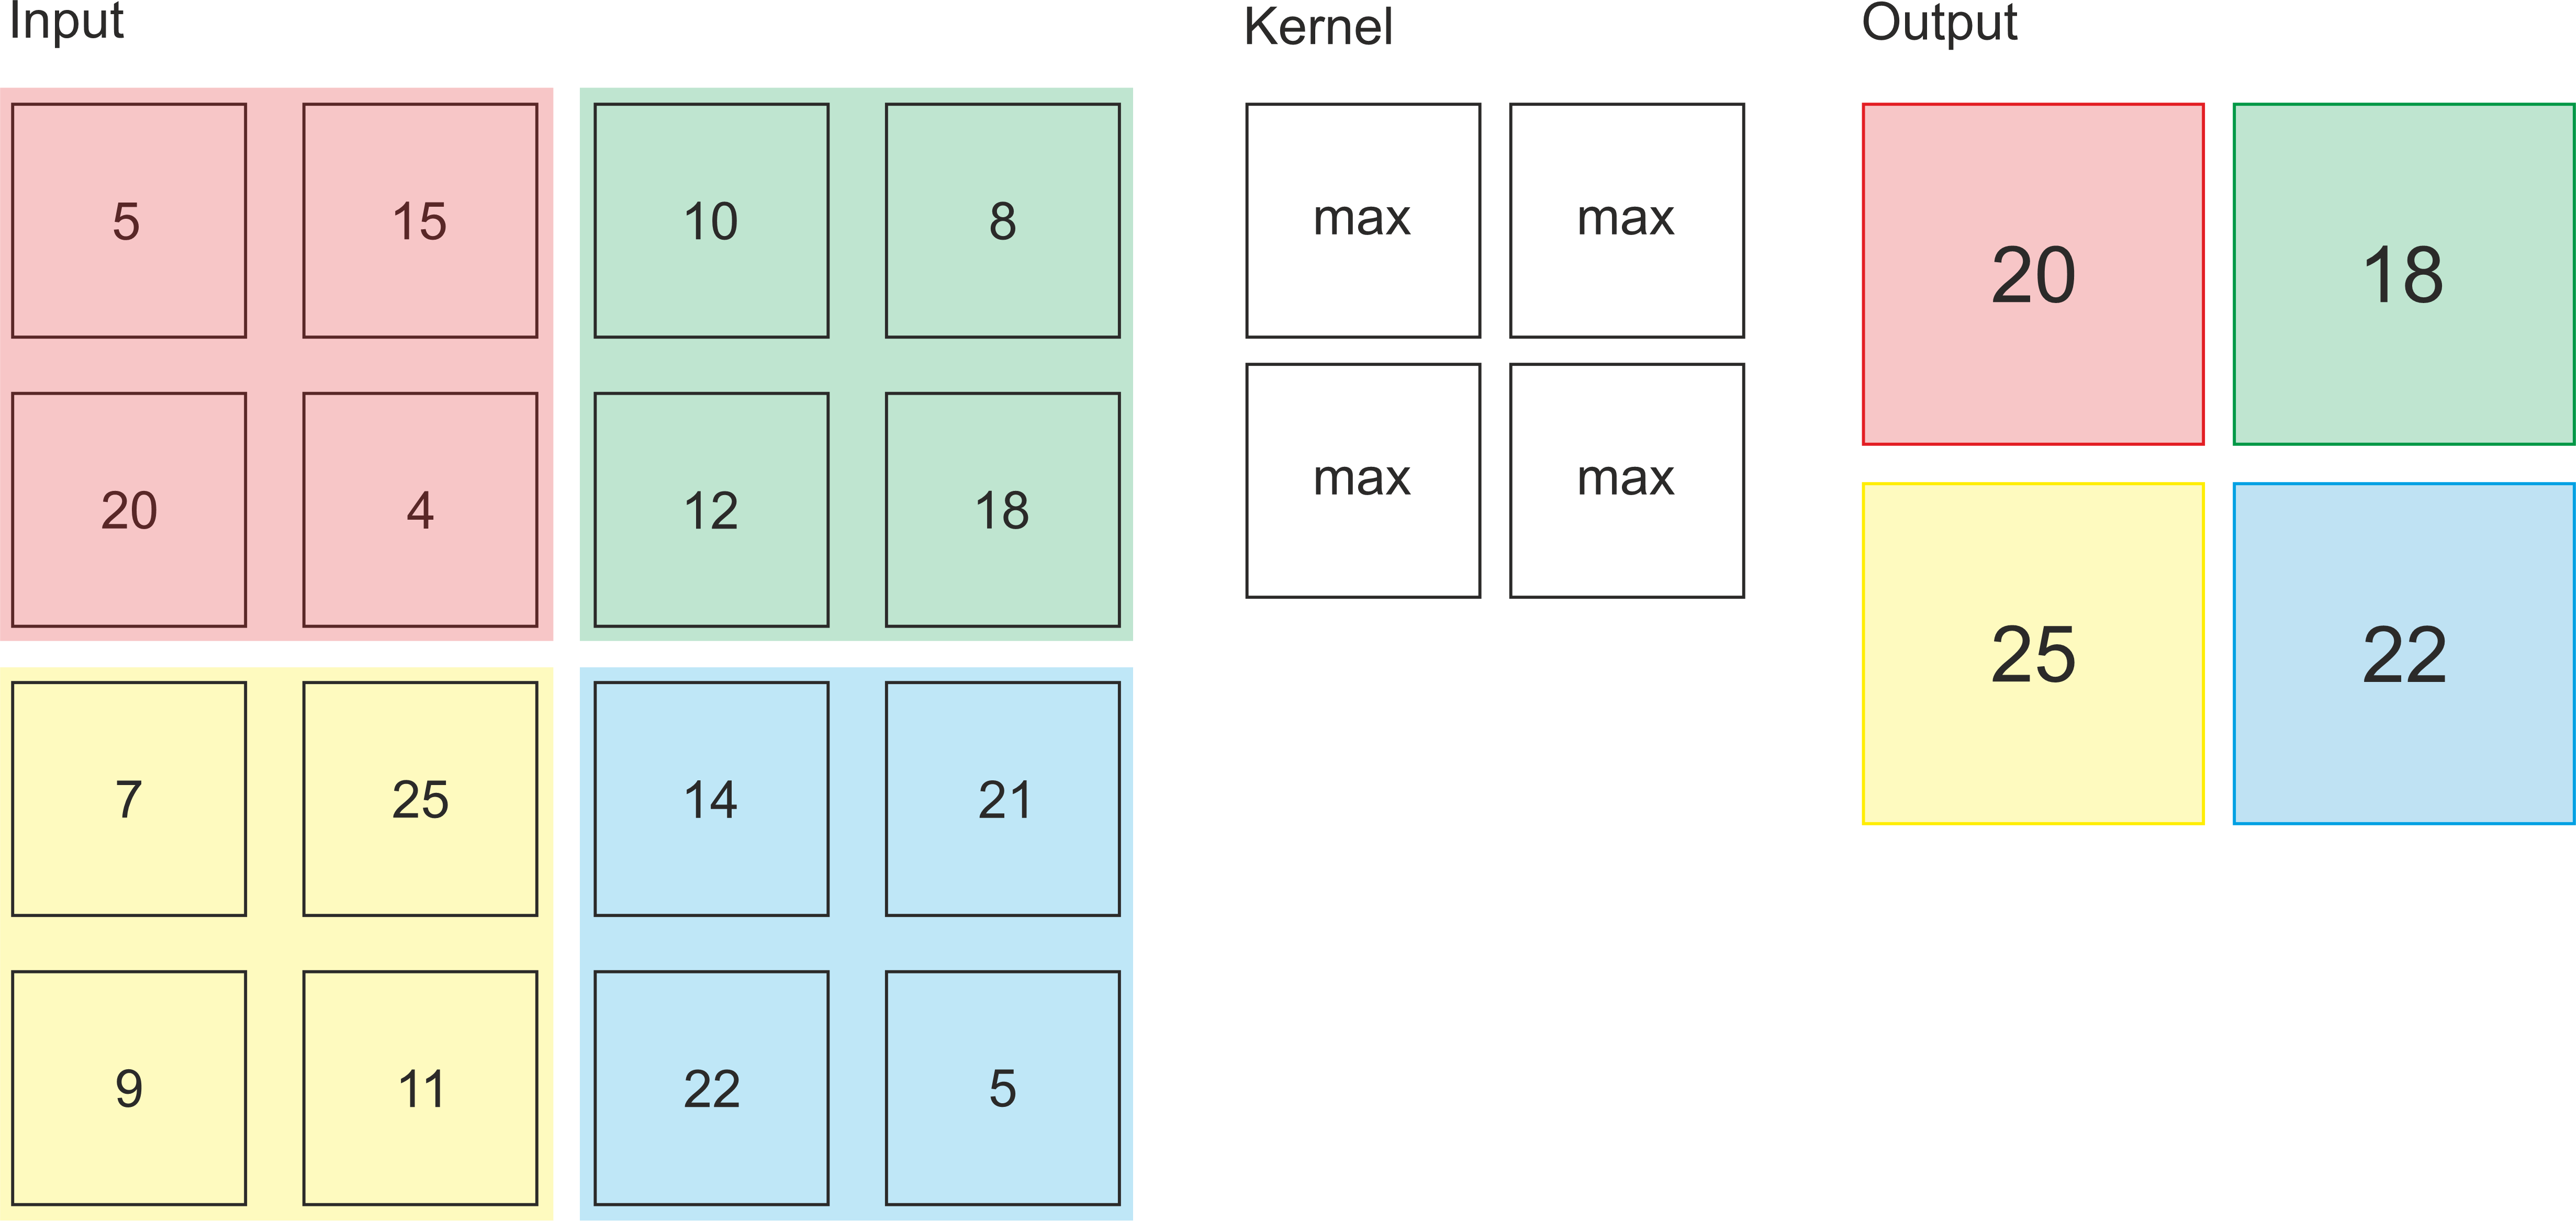
\includegraphics[width=.7\textwidth]{images/maxpooling.png}
    \caption{An example of max pooling.}
    \label{img:maxpool0}
\end{figure}

\subsubsection{Fully-connected layer}
Fully connected (FC) layers in CNN are identical to layers in a standard neural network. They consist of neurons that have no connection to each other within one layer, but each neuron from the previous layer is connected to each neuron in the following layer \cite{Goodfellow-et-al-2016}.

The structure of neurons in FC layers is no longer organized in 3 dimensions instead inputs and outputs are 1D vectors. Feature maps fed to a fully-connected layer, therefore, need to be flattened to one dimension.

While in standard neural networks, each layer is fully-connected, in CNN only the last layers that are responsible for calculating the class scores are fully-connected \cite{standford}.

%\section{Space object recognition} \label{sec:spacerecognition}
Object recognition refers to a series of computer vision tasks, whose goal is to identify objects on images. It consists of two separate tasks: object localization and classification. 
The first step of object recognition is to find all objects present in the image, which is the goal of the object localization task. The algorithm outputs the location of the object as well as the bounding box encapsulating the object. Each object is then assigned a label that defines the class that the object belongs to. This is called classification. 
%Next, features from each object need to be extracted. This can be done by means of traditional or deep learning methods. Based on these features, each object is assigned a label that defines the class that the object belongs to. This is called classification. 

%Object recognition is used in many areas of life. 
%% nieco kde sa to pouziva a potom ze sa to pouziva aj v astronomical field

In this chapter, we will talk about various approaches to object recognition through astronomical images or features extracted from them. %We will focus on two main things: the type of data and the proposed method. 

\subsection{Traditional methods}
For many years traditional analytical methods were used for object recognition. These methods relied on astronomers‘ knowledge of the given task and were designed for specific types of space objects. 

\subsubsection{On-orbit recognition of resident space objects by using star trackers}
The main goal of the article \cite{SPILLER2020478} was to evaluate the possibility of using star trackers to track resident space objects (RSO) in space. For this purpose, they developed an algorithm that could operate on board with limited computational performance and memory.
With this in mind, the algorithm could not be based on machine learning as this would be computationally demanding. 

In order to test the proposed algorithm, synthetic images needed to be generated using their own star-tracker hardware simulator. 
The simulator consists of two modules:
\begin{itemize}
    \item Sky and spacecrafts input generator
    \item High-fidelity image generator

\end{itemize}

The goal of the first block is to simulate the sky, stars, and RSOs. The sky simulation is performed using a star catalog while considering the position and orientation of the sensor as well as optical and geometric characteristics. A similar procedure is followed when simulating real RSOs, but using the catalog with orbiting RSOs instead of the star catalog. Another way of simulating RSOs is to use the grid method, which simulates fictitious RSOs. 
The second block is used to make the image realistic. The block receives the list of stars and RSOs with their position and magnitude. Using this data as well as some additional information regarding noises, optical, geometrical, and electronic characteristics of the sensor, the block produces high fidelity synthetic images. 

When it comes to the developed algorithm, the first step is to identify objects of interest from the background. After the identification of objects is complete, a list of objects and their positions is produced for every image. 
The algorithm is then given pairs of images and compares each object on the first image to each object in the second image. Based on some predetermined conditions regarding their position, distance, velocity, and density, objects are matched. This means that the object in the first image is the same object in the second image. The algorithm performs this comparison for a series of pairs of images and as a result, the object is being tracked.

This method was mainly developed to track moving objects in space-based observations. In this situation, RSOs usually appear as streaks and the algorithm was optimized for this scenario. However, this poses a disadvantage since point-like objects are not recognized well and diffuse sources are considered background noise. 

\subsection{Machine learning methods}
With an increase in the amount of data, the traditional methods weren't fast and robust enough. Machine learning methods were able to tackle this issue, by learning on their own. Extracting knowledge from a large amount of data allows them to find patterns in data that may not be visible to humans. This way they can outperform even the best traditional methods \cite{Goodfellow-et-al-2016}.

 
\subsubsection{Galaxy morphology classification using automated machine learning} 
In \cite{REZA2021100492}, multiple machine learning algorithms were tested with an aim to classify galaxies into four types. The study was conducted in order to assess the possibility of using ML for future surveys. 

Dataset used to train models contained more than 304 000 samples of galaxies of different types (spirals, ellipticals, mergers, and stars). Feature vectors were obtained from SDSS (Sloan Digital Sky Survey) and their extraction wasn't explained since that is not the main subject of the article. %Feature vector included features such as fiber, model and Petrosian colors, axis ratio, degree of ellipticity, and others. Explanation of each feature is provided in the mentioned article \cite{REZA2021100492} and will not be done here since they are not relevant to this thesis. 

Five different ML methods were chosen for the article - Decision trees, Random Forest, ExtraTrees, K-nearest neighbors, and Artificial Neural Network. Before the data was fed to any model, PCA was performed on feature vectors to reduce their dimensionality. As a result, 25 most significant features were used from the original feature vector of size 62. As usual, models were trained on the training set and hyperparameters were tuned on the separate validation set. 
Evaluating the models on the testing set and comparing the accuracy showed that ANN had the best results. Even though the overall accuracy of the ANN was the best, the accuracy of minority class samples showed poor results. In this case, ensemble methods like a combination of ExtraTrees with Random Forest performed much better. In conclusion, we can say that using a balanced dataset with a large number of samples could prove to be useful when working with ANN. 




\subsubsection{Applications of neural networks to object detection and star/galaxy classification}
%https://academic.oup.com/mnras/article/319/3/700/1073630?login=false
In the article, \cite{Andreon2000}, the developed package called Neural extractor (NExt) was presented. The package can perform object detection and star/galaxy classification. The authors used three different NNs for each specific task: data reduction, detection, and classification. 

For the training, validation, and testing, the subset of the IP92 catalog \cite{1992ApJS} was used. To train the detection part of the algorithm, the best solution was to use around 10 subimages 50x50 pixels wide. To test the performance of the detection and classification networks, 4819 and 460 objects from the catalog were chosen, respectively.

The first step of the package included the detection of desired objects. This task was performed as a classification of pixels into background and object class. First, the non-linear PCA NN was applied to the image, which reduced the redundant information in nearby pixels. Transformed values of the pixels were then fed to unsupervised NN. Multiple different models were tested and the best performing one was a multi-layer neural gas network with a running window of size 3 or 5. 
This network aimed to classify pixels into background or object class. This was done in an unsupervised matter and the network has split pixels into multiple classes. One of the classes could be described as a background, whereas the others described different kinds of astronomical objects and were later merged to form an object class. After the segmentation, the overlapping objects were detected and deblended.
The second step included feature extraction and the star/galaxy classification. Considering feature extraction, multiple features were measured, and through the sequential backward elimination strategy, the best-performing ones were selected. These features were then used to train MLP to perform the final task of star/galaxy classification. 

To test the performance of the proposed method, the authors compared the results to the best performing package at the time (SExtractor \cite{sextractor}). Considering the detection phase of the algorithm, the proposed method was as effective as the SExtractor in the detection of true objects. For the classification phase, the NExt performed better than the SExtractor, with only 28 errors compared to 41 for the SExtractor from the total of 480 objects. 

It wasn't explicitly mentioned in the article but according to pictures, this method considers the only point-like appearance of the stars. This poses a huge disadvantage in our case since the space debris usually appears as streaks during the sidereal tracking.  



\subsubsection{Deblending and classifying astronomical sources with Mask R-CNN deep learning}
In \cite{Burke2019}, a network based on Mask Region-based CNN (Mask R-CNN) framework is used to detect, classify and deblend star and galaxy sources. 

The network is trained, validated, and tested using simulated images generated by The Photon Simulator. The simulator generates 512x512 three-band images, where each image contains around 150 objects. For the training set, 1000 images were simulated, which is approximately 150 000 astronomical sources. The validation and testing set contains 250 and 50 simulated images, respectively. 

The Mask R-CNN \cite{maskrcnn2017} comes from a family of region-based CNN frameworks, that specialize in the task of object recognition. The architecture of the R-CNN framework could be summarized as multiple subnetworks, where each has its own specific task. The backbone of the framework is a deep CNN, whose goal is to extract features from the image. The region proposal network finds regions in the image and the type of object in the area. At the end of the framework, there are 2 subnetworks, one predicts the type of object in the proposed region, and the other outputs the bounding box of the object. Mask R-CNN is an extension of R-CNN frameworks, with additional subnetwork for instance segmentation.
In the article, the backbone used for Mask R-CNN is a Resnet with 101 layers. Transfer learning was used to improve the speed of the training process, with initial weights trained on the MS COCO dataset.  

The network was tested on simulated images and achieved a precision of 92 \% on star sources and 98 \% on galaxies. Results also revealed that the network performs significantly better with small sources, which could be due to a few large examples in the training set. 





%%%%%% does not need to cite

% articles about streaks
% https://cds.cern.ch/record/1707548/files/978-1-4939-0629-1_BookBackMatter.pdf
% https://conference.sdo.esoc.esa.int/proceedings/neosst1/paper/444/NEOSST1-paper444.pdf
% https://www.aanda.org/articles/aa/full_html/2020/12/aa37765-20/aa37765-20.html
% https://reader.elsevier.com/reader/sd/pii/S0094576521001211?token=93F8903DF4BF28EC64C9DE8B86B59D6C71136A835A32EB40977BA9A729EB5DAFCCF2437D4B81A5717C58E2BC46B52704&originRegion=eu-west-1&originCreation=20210804182521

% articles about astronomical imagining
% https://link.springer.com/chapter/10.1007/978-3-319-21969-1_37
% https://subarutelescope.org/staff/guyon/15teaching.web/00AstrOptics.web/AstrOpt_01fund.pdf

% articles about ccd artifacts
% https://arxiv.org/pdf/1601.07182.pdf
% https://mwcraig.github.io/ccd-as-book/01-00-Understanding-an-astronomical-CCD-image.html

% articles about noises
% https://hamamatsu.magnet.fsu.edu/articles/ccdsnr.html
% https://www.mssl.ucl.ac.uk/www_detector/ccdgroup/optheory/darkcurrent.html
% https://camera.hamamatsu.com/jp/en/technical_guides/calculating_snr/index.html






